\chapter{Modellazione concettuale} \label{chap:modellazione_concettuale}
	
	A partire dalla pseudo-narrazione derivante dalla descrizione, dagli obiettivi di questo progetto e dall'analisi dei \textit{dataset} utilizzati si può ottenere uno schema concettuale che, attraverso una serie di entità e le relazioni tra esse, possa modellare dettagliatamente la realtà che ci proponiamo di analizzare.\\
	Gli obiettivi da tener presente nella costruzione dello schema concettuale sono: da una parte la necessità di soddisfare i requisiti utente; dall'altra la necessità di consistenza dello schema concettuale con gli schemi delle sorgenti operazionali.\\
	L'approccio metodologico alla progettazione concettuale utilizzato è l'approccio guidato dai dati: lo schema concettuale viene cioè definito in funzione della struttura delle sorgenti stesse, evitando così il complesso compito di stabilire il legame con esse a posteriori.
	
	\begin{figure}[h!]
		\centering
			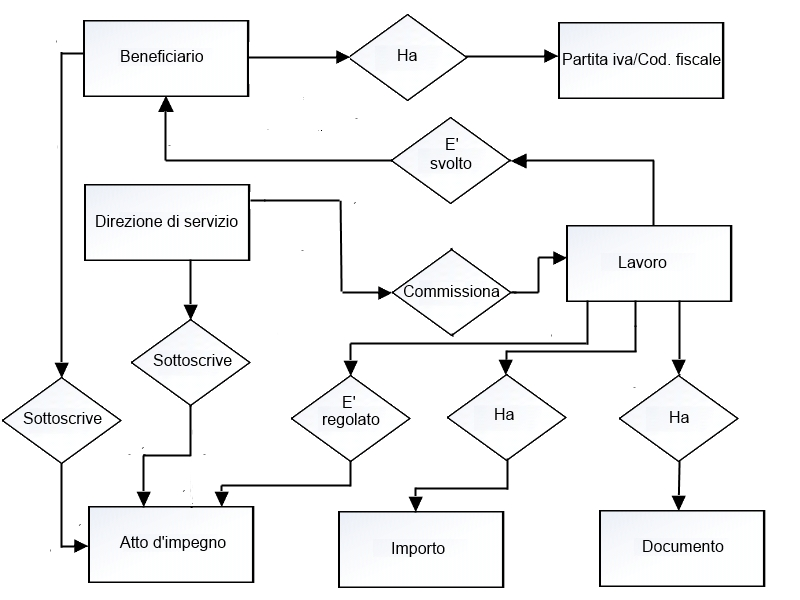
\includegraphics[scale=0.5]{schemaconcettuale.jpg}
		\caption{Schema-concettuale.}
		\label{fig:schemaconcettuale}
	\end{figure}
	
	Una modellazione di questo tipo fornisce inoltre le basi per la costruzione di un'ontologia e una conseguente interrogazione dei dati da un punto di vista semantico.\\
	Il passaggio successivo consiste nell'attribuzione di un \textbf{URI} (\textit{Uniform Resource Identifier}) alle entità coinvolte nello schema, in modo tale da creare una correlazione tra i riferimenti del modello e la posizione reale dei dati.\\
	\\
	Lo schema concettuale presentato può essere successivamente tradotto in uno schema entità-relazione più appropriato, che prende il nome di \textit{Dimensional Fact Model}. Questo modello concettuale è specificatamente concepito per fungere da supporto alla progettazione di un \textit{Data Warehouse} e può essere considerato come una specializzazione del modello multidimensionale.\\
	Come si può osservare nella Figura \ref{fig:schemariconciliato}, la rappresentazione generata dal DFM consiste in un insieme di schemi di fatto: gli elementi di base modellati sono i fatti stessi, le misure e le dimensioni.
	
	
	\begin{figure}[h!]
		\centering
			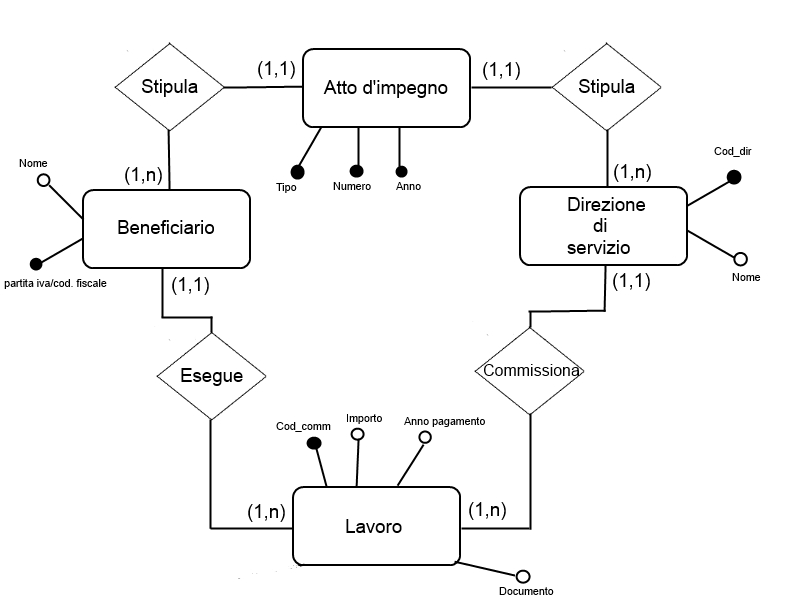
\includegraphics[scale=0.65]{schemariconciliato.jpg}
		\caption{Schema riconciliato.}
		\label{fig:schemariconciliato}
	\end{figure}
